\documentclass[addpoints]{exam}
%\documentclass[addpoints,answers]{exam}
\usepackage{url}
\usepackage{times}
\usepackage{epsfig}
\usepackage{listings}
\usepackage{mathtools}
\lstset{
basicstyle=\small\ttfamily,
columns=flexible,
breaklines=true,
moredelim=[is][keywordstyle]{@@}{@@},
moredelim=[is][\bfseries\underbar]{__}{__}
}

\lhead{\ifcontinuation{Question \ContinuedQuestion\ continues\ldots}{}}
\chead{ECE 422 / CS 461, Final Exam}
\rhead{Monday, May 9th, 2016}
\lfoot{Points: \makebox[.5in]{\hrulefill} / \pointsonpage{\thepage}}
\cfoot{\thepage\ of \numpages}
\rfoot{NetID:\enspace\makebox[1.5in]{\hrulefill}}
%\rfoot{\netid}

\qformat{\thequestiontitle\dotfill \emph{\totalpoints\ points}}

\begin{document}

\begin{titlepage}
  \vspace*{\fill}
  \begin{center}
    \Large\textbf{ECE 422 / CS 461, Final Exam}\\
    \large\textit{Monday, May 9th, 2016}\\
  \end{center}
  \vspace{.5in}
  \par\large{Name:}\hrulefill\\
  \par\large{NetID:}\hrulefill\\
  \vspace{.5in}
  \begin{itemize}
  \item Be sure that your exam booklet has \numpages\ pages.
  \item Absolutely no interaction between students is allowed.
  \item Show all of your work.
  \item Write all answers in the space provided.
  \item Closed book, closed notes.
  \item No electronic devices allowed.
  \item You have \textbf{THREE HOURS} to complete this exam.
  \end{itemize}
  \vspace*{\fill}
\end{titlepage}
\newpage 

\begin{center}
  \vspace*{\stretch{1}}
  \gradetable[v][pages]
  \vspace*{\stretch{1}}
\end{center}
\newpage

\begin{questions}

\titledquestion{Question \thequestion: Multiple Choice}

%The line below is invalid since you will not solely be circling answers
%\textbf{For each question, circle all that apply.}

\begin{parts}

\part[2] %Gene
What are booter services?

\begin{choices}
\choice Services to track where the attackers are
\choice Services that help customers to boot their laptops
\correctchoice Services that help perform DDoS attacks
\choice Services to filter packets that are coming into the network
\end{choices}

\part[2] %Gene

Internet Protocol (IP) is secure by itself since there is a checksum field in the IP header.

\begin{choices}
\choice True
\correctchoice False
\end{choices}

\part[2] %Matt

What aspect(s) of security are SSL and TLS designed to ensure? (Select all that apply)

\begin{choices}
\correctchoice Authentication
\choice Availability
\correctchoice Confidentiality
\correctchoice Integrity
\end{choices}

\part[2] %Matt

What are the primary issues with DNS that stem from lack of authentication? (Select all that apply)

\begin{choices}
\choice IP Spoofing
\correctchoice Cache Poisoning
\correctchoice DNS Spoofing
\choice Resource exhaustion
\end{choices}

\part[2] %Matt

Off-The-Record Messaging provides perfect forward secrecy.

\begin{choices}
\correctchoice True
\choice False
\end{choices}

\part[2] %Lawrence

MAC flooding and ARP spoofing are two attacks that take place at which layer?

\begin{choices}
\choice Network
\choice Application
\correctchoice Link
\choice Transport
\choice Session
\end{choices}

\part[2] %Lawrence

Stateless firewalls are harder to scale than stateful firewalls because of the need to maintain a static filter list.

\begin{choices}
\choice True
\correctchoice False
\end{choices}

\part[2] %Tong

How might one hide data on a hard drive? (Select all that apply)

\begin{choices}
\correctchoice Steganography
\choice Machine Learning
\correctchoice Cryptography
\choice Anomaly Detection
\end{choices}

\part[2] %Tong

Which of the following is an effective way to defend against IP spoofing?
\begin{choices}
\choice Firewall
\choice IDS
\correctchoice IPsec
\choice HTTPS
\end{choices}

\pagebreak

\part[2] %Tong

In modern OSes where initial sequence numbers (ISN) are highly randomized, TCP hijacking is nearly impossible.
\begin{choices}
\choice True
\correctchoice False
\end{choices}

\part[2] %Shivam

Tor provides encryption between the exit node and the destination. 
\begin{choices}
\choice True
\correctchoice False
\end{choices}

\part[2] %Siddharth

If you receive an email from a known company that says ``Click this link to reset your bank password'', what type of attack is likely being used?  
\begin{choices}
\choice Man-in-the-middle
\correctchoice Spear Phishing
\choice IP spoofing
\choice DDoS
\end{choices}

\part[2] %Siddharth

Which of the following describes a decoy system designed to be attacked? 
\begin{choices}
\correctchoice Honeypot
\choice Rootkit
\choice Trojan Horse
\choice None of the above
\end{choices}

\part[2] %Siddharth

DoS affects which of the areas of the CIA triad? 
\begin{choices}
\choice Confidentiality
\choice Integrity
\correctchoice Availability
\choice Authenticity
\end{choices}

\part[2] %Dhruv

Worms are able to spread without human intervention.
\begin{choices}
\correctchoice True
\choice False
\end{choices}

\part[2] %Dhruv

You use Tor to access a destination address. Where along the path is your identity known?
\begin{choices}
\correctchoice Entry Node
\choice Intermediate Node
\choice Exit Node
\choice Destination
\end{choices}

\part[2] %-HB
There are \textbf{two} types of paradigms in Intrusion Detection which were discussed in the lecture. What are they? (Select all that apply)

\begin{choices}   
\choice Network Intrusion Detection Systems
\correctchoice Misuse Detection Intrusion Detection Systems
\choice Protocol Based Intrusion Detection Systems
\correctchoice Anomaly Detection Intrusion Detection Systems
\end{choices}

\end{parts}

\pagebreak

\titledquestion{Question \thequestion: Short Answer}

\begin{parts}

\part[3] %-Gene
Describe the 3 primary stages of a botnet's lifecycle.

\begin{solutionorbox}[1in]

Propagation - acquiring members through worms/trojan horses\\
Communication - phone-back to attacker\\
Attacks - Networking Attacks (DDoS, phishing, spam, etc)

\end{solutionorbox}

\part[3] %-HB
A pcap trace below was captured after a networking attack. The Victim's ip address is 10.0.1.1. What kind of attack is this? Explain how adversary executed this attack.

%example based on http://www.ufsdump.org/papers/uuasc-november-ddos.html
\begin{verbatim}
05:31:39.435997 IP 10.0.0.1 > 10.0.1.1: icmp 16: echo reply seq 9472
05:31:39.436668 IP 10.0.0.101 > 10.0.1.1: icmp 16: echo reply seq 9472
05:31:39.438082 IP 10.0.0.35 > 10.0.1.1: icmp 16: echo reply seq 9472
05:31:39.439051 IP 10.0.0.92 > 10.0.1.1: icmp 16: echo reply seq 9472
05:31:39.439357 IP 10.0.0.108 > 10.0.1.1: icmp 16: echo reply seq 9472
05:31:39.441213 IP 10.0.0.6 > 10.0.1.1: icmp 16: echo reply seq 9472
...
\end{verbatim}

\begin{solutionorbox}[1in]

1 point: (ICMP) Smurf DOS attack\\
1 point: The adversary sends an ICMP requests (ping) to a broadcast IP address (e.g. 10.0.0.255).\\
1 point: The ICMP request src is spoofed to 10.0.1.1

\end{solutionorbox}

\part[3] %-HB
Explain what TCP SYN Flood attack is and suggest a solution to protect against the attack.

\begin{solutionorbox}[1.5in]

1 point: attacker makes multiple connections. (sends SYN packets)\\
1 point: server responds with ACK packets but attacker ignores.\\
1 point: server drops connection after certain threshold if ACK is never acknowledged by client.

\end{solutionorbox}

\part[2] %-HB
After the Heartbleed vulnerability was disclosed by OpenSSL in 2014, majority of large websites have swiftly reacted and patched the vulnerability. Meanwhile, there still remains some concerns. Explain two concerns which were mentioned in the lecture.

\begin{solutionorbox}[1.5in]

1 point: There are still large amount of websites which still use vulnerable version of OpenSSL.\\
1 point: Some websites patched but reuse old certificates and public and private key pairs.

\end{solutionorbox}

\pagebreak

\part[1] %-Zhengping
List an advantage of nondestructive entry over destructive entry.

\begin{solutionorbox}[0.5in]
1 point: Defeat intrusion detection
\end{solutionorbox}

\part[2] %-Zhengping
What does the security of TCP connections rely on? 

\begin{solutionorbox}[0.5in]   
2 points: Randomness of the initial sequence and acknowledgement numbers.
\end{solutionorbox}

\part[3] %Shivam
List the three different categories of security controls.

\begin{solutionorbox}[1in]

1 point: Management/Administrative Controls \\
1 point: Physical Controls \\
1 point: Technical/Logical Controls

\end{solutionorbox}

\part[2] %Dhruv
Mention one possible attack against onion routing and a possible solution against that attack.

\begin{solutionorbox}[1.5in]

1 point: Rubber-Hose cryptanalysis of mix operators\\
1 point: Mix servers in different countries\\
OR\\
1 point: Adversary operates all of the mixes\\
1 point: Have lots of mix servers\\
OR\\
1 point: Timing attack\\
1 point: Introduce delays

\end{solutionorbox}


\end{parts}

\pagebreak

\titledquestion{Question \thequestion: Crypto MP Question} % Due

\begin{parts}

\part[2]

In MP 3.2.1, we showed that MD5 is susceptible to length extension attack. Recall that SHA256 is a cryptographic hash function that uses Merkle-Damgard construction and produces digest of size 256 bits. \\

True or False: SHA256 is vulnerable to length extension attack.

\begin{choices}
\correctchoice True
\choice False
\end{choices}

\part[2]

In MP 3.2.1.1, we gave an example of MD5 length extension attack and described the structure of MD5 padding. Recall that MD5 processes messages in 512-bit blocks. Let $m_1$ be a message that is 20 bits long, and let $m_2$ be a message that is 532 bits long. \\

True or False: the MD5 padding for $m_1$ and $m_2$ have the same length when MD5 is applied to each message.

\begin{choices}
\correctchoice True
\choice False
\end{choices}

\part[3]

From part (b), would the \textbf{content} of the MD5 padding be the same for for $m_1$ and $m_2$? Briefly explain.

\begin{solutionorbox}[1in]
No, because the length of the unpadded message is included as part of the padding.\\
+2 No\\
+1 Explanation
\end{solutionorbox}

\part[3]

In MP 3.2.1.2, we asked you to conduct a length extension attack on an imaginary server API. Recall that the API verifies the integrity of the URL by using an authentication token of the form MD5(\emph{user's password} $\parallel$ \texttt{user=}.... [\emph{the rest of the URL starting from \texttt{user=} and ending with the last command}]). If the user's password is between 8-12 characters long, how many URLs must you construct to guarantee that at least one of them will be treated as valid by the server? Briefly explain.

\begin{solutionorbox}[1in]
5, because we need 1 URL for each possible password length.\\
+2 for correct number\\
+1 for correct explanation
\end{solutionorbox}

\part[3]

From part (d), if the token is instead computed as follow:\\

\emph{token} = MD5(\emph{MD5(user's password)} $\parallel$ \texttt{user=}.... )\\

Assume that the user's password is between 8-12 characters long. How many URLs must you construct to guarantee that at least one of them will be treated as valid by the server? Briefly explain.

\begin{solutionorbox}[1in]
1, because the MD5 hash of the passwords all have the same length.\\
+2 for correct number\\
+1 for correct explanation
\end{solutionorbox}

\pagebreak

\part[2]

In MP 3.2.4, you were asked to generate postscript files with different content that have the same MD5 hash. Recall that fastcoll is a program that can produce a pair of binary blobs that has the same MD5 hash under specific conditions. Assume that fastcoll always produce blobs that are compatible with postscript. What is the minimum number of times you need to run fastcoll to create 64 postscript files that have different content but have the same MD5 hash?

\begin{solutionorbox}[0.5in]
6
\end{solutionorbox}

\end{parts}

\pagebreak

% simons question goes here
\titledquestion{Question \thequestion: Network MP Question} % Simon

For all parts of this question, consider the following network topology.\\
Assume that the default firewall policy allows all traffic.
\begin{center}
    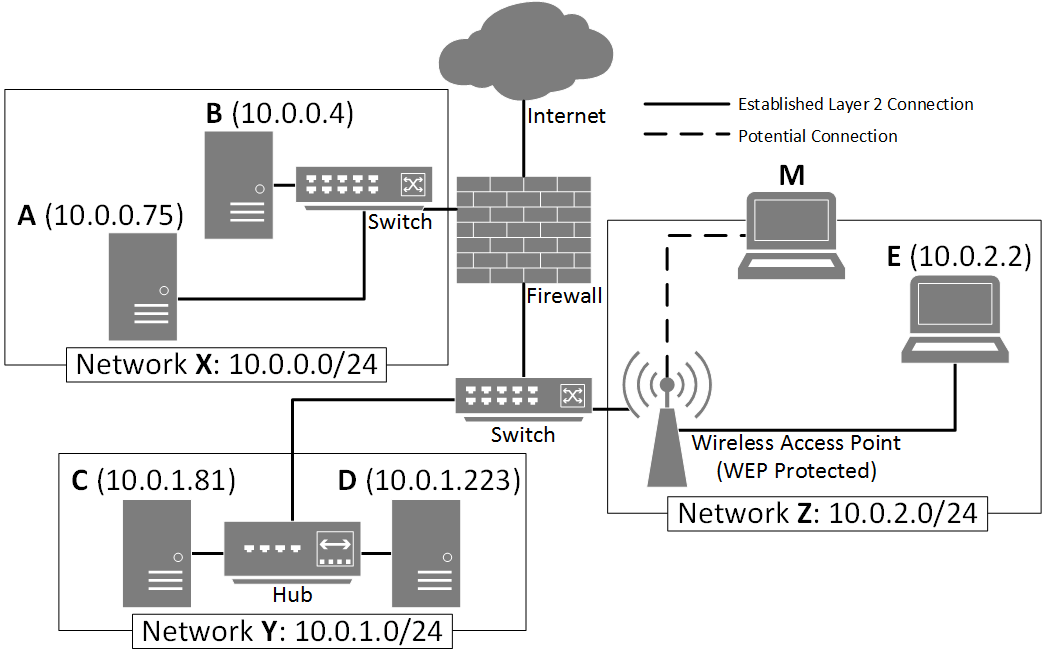
\includegraphics[scale = 0.55]{topology} \\
\end{center}

\begin{parts}

\part[1]
Assume that there is an active unencrypted TCP session between Hosts A and C and that every host on the network knows the IP address of A and C.
\\
Which other host(s) on the network can eavesdrop on this communication by performing passive sniffing only?

\begin{solutionorbox}[0.5in]
D\\
+1 correct
\end{solutionorbox}

\part[2]
Assume that there is an active unecrypted TCP session between Hosts B and C and that every host on the network knows the IP address of B and C.\\
\\
What technique can Host A use to eavesdrop on this communication? Name the technique and briefly describe it.

\begin{solutionorbox}[1in]
MAC flooding, filling up switch's memory with random MAC addresses; ARP spoofing, changing victim's ARP table\\
+1 correct name\\
+1 correct explanation
\end{solutionorbox}

\pagebreak

\part[4]
Assume that there is an active unencrypted TCP session between Hosts B and E and that Host M is not part of any network or associated with the wireless access point.

\begin{subparts}
\subpart
How should Host M's wireless adapter be configured to eavesdrop on this communication?
\begin{solutionorbox}[0.5in]
monitor mode\\
+1 correct
\end{solutionorbox}

\subpart
Host M detects other wireless network activities nearby.\\
\\
What two pieces of wireless network information can be provided to airodump-ng so that only the packets from Network Z are captured?
\begin{solutionorbox}[0.5in]
BSSID (or MAC address of AP), channel number\\
+1 each correct name
\end{solutionorbox}

\subpart
When inspecting the captured packets with Wireshark, the user of Host M is unable to see the contents because they are encrypted by WEP.\\
\\
Which wireless network information does the user need to see the plaintext version of the payload?
\begin{solutionorbox}[0.5in]
WEP key\\
+1 correct
\end{solutionorbox}

\end{subparts}

\pagebreak

\part[4]
Consider the following packet trace from the network:\\

{
\centering
\begin{tabular}{|l|l|l|l|l|l|}
\hline
\textbf{src\_ip}  & \textbf{src\_port}  & \textbf{dst\_ip}  & \textbf{dst\_port}  & \textbf{tcp\_flags} \\ \hline
\multicolumn{5}{|c|}{...} \\ \hline
10.0.0.4          & 21                  & 10.0.1.223        & 50678               & {[}SYN, ACK{]}      \\ \hline
10.0.1.223        & 50678               & 10.0.0.4          & 21                  & {[}ACK{]}           \\ \hline
10.0.0.4          & 21                  & 10.0.1.223        & 50678               & {[}PSH, ACK{]}      \\ \hline
\multicolumn{5}{|c|}{...} \\ \hline
10.0.0.4          & 20                  & 10.0.1.223        & 43583               & {[}SYN{]}           \\ \hline
10.0.1.223        & 43583               & 10.0.0.4          & 20                  & {[}SYN, ACK{]}      \\ \hline
10.0.0.4          & 20                  & 10.0.1.223        & 43583               & {[}ACK{]}           \\ \hline
\multicolumn{5}{|c|}{...} \\ \hline
10.0.0.4          & 20                  & 10.0.1.223        & 43583               & {[}FIN, ACK{]}      \\ \hline
10.0.1.223        & 43583               & 10.0.0.4          & 20                  & {[}FIN, ACK{]}      \\ \hline
10.0.0.4          & 20                  & 10.0.1.223        & 43583               & {[}ACK{]}           \\ \hline
\multicolumn{5}{|c|}{...} \\ \hline
10.0.1.223        & 50678               & 10.0.0.4          & 21                  & {[}FIN, ACK{]}      \\ \hline
10.0.0.4          & 21                  & 10.0.1.223        & 50678               & {[}FIN, ACK{]}      \\ \hline
10.0.1.223        & 50678               & 10.0.0.4          & 21                  & {[}ACK{]}           \\ \hline
\multicolumn{5}{|c|}{...} \\ \hline
\end{tabular}\\
}

\vspace{.2in}

Assuming that this is a trace of FTP file transfer, answer the following questions:
\begin{subparts}
\subpart
What is the IP address of the FTP server?

\begin{solutionorbox}[0.5in]
10.0.0.4\\
+1 correct
\end{solutionorbox}

\subpart
What port number did the server use to transfer data (i.e. FTP-DATA port)?

\begin{solutionorbox}[0.5in]
20\\
+1 correct
\end{solutionorbox}

\subpart
Is this FTP transfer done in active or passive mode? Give one reason why you came to this conclusion.
\begin{solutionorbox}[1in]
active mode, because FTP-DATA is port 20 or data transfer is initiated by the server.\\
+1 correct answer\\
+1 correct explanation
\end{solutionorbox}

\end{subparts}

\pagebreak

\part[3]
Based on the diagram at the beginning of Question 4, create inbound firewall rules that satisfy the following conditions:
\begin{itemize}
\item Deny all inbound traffic to Network X by default.
\item Allow inbound traffic to Network X for HTTP.
\item Allow Network Y to SSH to Network X.
\end{itemize}

\vspace{.05in}

Fill in the table following the directions below:
\begin{itemize}
\item You may or may not need to use all rows.
\item Assume that rules are processed from the top down.
\item For \textbf{Source} and \textbf{Destination} columns, you may write either the network name or its IP address range in CIDR notation to specify a range of IP addresses or a network.
\item For \textbf{Application} column, you may write either the service name or its port number.
\end{itemize}

{
\centering
\begin{tabular}{|p{4cm}|p{4cm}|p{3cm}|p{3cm}|}
\hline
\textbf{Source} & \textbf{Destination}  & \textbf{Application}  & \textbf{Action} \\      \hline
                &                       &                       &                 \\[2ex] \hline
                &                       &                       &                 \\[2ex] \hline
                &                       &                       &                 \\[2ex] \hline
                &                       &                       &                 \\[2ex] \hline
\end{tabular}\\

}
\vspace{.1in}

Example (does not apply to our topology):\\

{
\centering
\begin{tabular}{|p{4cm}|p{4cm}|l|p{2cm}|p{1cm}|}
\hline
\textbf{Source}             & \textbf{Destination}  & \textbf{Application}  & \textbf{Action} \\ \hline
Network W (or 10.0.7.0/24)  & 10.0.4.4              & SMTP (or 25)          & Allow           \\ \hline
\end{tabular}\\
}

\vspace{.1in}

\begin{solution}[3in]

+1 for each correct row\\
-0.5 if Deny all is not the first row\\
-1 for each of other incorrect rows\\

{
\centering
\begin{tabular}{|l|l|l|l|l|}
\hline
\textbf{Source}   & \textbf{Destination}  & \textbf{App}    & \textbf{Action} \\ \hline
Any               & X or 10.0.0.0/24      & Any             & Deny            \\ \hline
Any               & A or 10.0.0.75        & HTTP or 80      & Allow           \\ \hline
Y or 10.0.1.0/24  & A or 10.0.0.75        & SSH or 22       & Allow           \\ \hline
\end{tabular}\\
}

\end{solution}

\end{parts}


\pagebreak

\titledquestion{Question \thequestion: Forensics MP Question} % -Leslie

Another incident has happened around the same time as the murder introduced
in MP5, near Halloween, 2015. An hour later, police officers were able to obtain 
multiple hard disks on site. Those were sent out to the digital forensics 
department who found that all but two hard disks were wiped clean. One of the 
system's users was ``hacker'' and another system's user was ``security.expert''. 

Bob was recently hired in the digital forensics team and was given these as his 
first case to investigate. As he started to investigate, he was so excited and 
booted the hard disk on a machine, selected a disk partition, and started to 
explore. He navigated through the system's directories, opened a few log files 
to look for the relevant evidence, and ran some commands. Then, he realized
something was wrong.

Fortunately, a more experienced expert, Cathy, duplicated the original
disk images before Bob started investigating. Through Autopsy, she
extracted a few files that might be relevant to the case. \textbf{Part
of the files are provided on the next page(s)} which are based on
the same time zone setting as the setting of the user's machine.

\begin{parts}

\part[2]
What are the results that Bob's action can lead to? List two different things that can happen to the evidence during live analysis.

\begin{solutionorbox}[1in]
[1 point] tampering of the data: e.g. last accessed time of the file gets changed, bash history gets overwritten
[1 point] suspect may have pre-setup the partition to prevent from live analysis (obfuscate with other OS partition, disk wiping etc.)
(optional) attacking of the system is maybe needed to log on
\end{solutionorbox}

\part[1]
Where in the file system can you find installed OS kernel version number information?

\begin{solutionorbox}[0.5in]
/proc/version
\end{solutionorbox}

\part[2]
What was the e-mail account used by the hacker? What time did the hacker write the last email? Write the time in CST in MMDDHHmm (MM=Month, DD=day, HH=hour, mm=minute) format.

\begin{solutionorbox}[0.5in]
[1 point] hacker.1996@gmail.com [1 point] 2015-10-30 17:25
\end{solutionorbox}

\part[2]
Do you find any trace of an attack on hacker's machine? If so, what is the IP address of the attacker?

\begin{solutionorbox}[0.5in]
[1 point] no attack and [1 point] unknown
\end{solutionorbox}

\part[2]
How many IP addresses were assigned to the hacker's system?

\begin{solutionorbox}[0.5in]
2 IP addresses. /var/log/syslog contains the IP address assigned to the machine. There are 3 IP addresses requested but only 2 were acknowledged.
\end{solutionorbox}

\part[2]
Let's assume that security.expert has successfully made a connection to hacker's system. When security.expert connected to hacker's system remotely for the first time, the server configured a public and private key pair as a fingerprint. It is generated once per host when the server is configured and this is used to identify the host. What algorithm was used to generate this key pair?

\begin{solutionorbox}[0.5in]
RSA.
\end{solutionorbox}

\pagebreak

\part[1]
Let's say you have recovered an unallocated file using a tool called extundelete. You have opened the file and started to wonder if the content has been modified from the original file. How can you verify whether the recovered file hasn't been overwritten by other data?

\begin{solutionorbox}[1in]
Compare the hash values (MD5, SHA256) of the file and compare with the hash value from metadata of the unallocated file.
\end{solutionorbox}

\end{parts}

\pagebreak

\begin{lstlisting}
__<Hard Disk of hacker>__
@@File path: /etc/hosts@@
127.0.0.1   localhost
127.0.1.1   hacker-personal

@@File path: /etc/lsb-release@@
DISTRIB_ID=Ubuntu
DISTRIB_RELEASE=14.04

@@File path: /etc/localtime@@
EST5EDT,M3.2.0,M11.1.0

@@List of files in file path: /etc/ssh@@
sshd_config.factory-defaults    ssh_host_ecdsa_key          ssh_host_ed25519_key.pub
ssh_host_dsa_key                ssh_host_ecdsa_key.pub      ssh_host_rsa_key
ssh_host_dsa_key.pub            ssh_host_ed25519_key        ssh_host_rsa_key.pub

@@File path: /home/hacker/.ssh/known_hosts@@
|1|v1lijAzbD0R3YEIeI60YOZcLr6w=|/M4HmYBQ7X3IVbXIAoBDutzyN0g= ecdsa-sha2-nistp256 AAAAE2VjZHNhLXNoYTItbmlzdHAyNTYAAAAIbmlzdHAyNTYAAABBBOLvT/D    S/3fb+OrtW+JuCXJjtV+XcqhPrRQbCWBrE+rSL2wLx47p5jJ3o52c0dEkHuFT8yuJ0upDsoKAFHs14iA=

@@File path: /home/hacker/.mozilla/firefox/places.sqlite@@
<Access Time>   2015-10-30 19:01:00
<Modify Time>   2015-10-30 19:01:00

<Date Accessed> <Strings (Contents)>   
Oct 30 17:15:00 https://mail.google.com/
Oct 30 17:15:24 https://mail.google.com/mail/u/0/#inboxInbox (54) - hacker.1996@gmail.com - Gmail...
Oct 30 18:15:18 https://mail.google.com/mail/u/0/#search/security.expert
Oct 30 18:15:39 https://mail.google.com/mail/u/0/#search/from%3A+security.expert%40gmail.com/14d2816b7a04c3ff Hey! - security.expert@gmail.com - Gmail...
Oct 30 18:25:31 https://mail.google.com/mail/u/0/#inbox?compose=new
Oct 30 18:25:49 https://mail.google.com/mail/u/0/#inbox?compose=new=24987sdf98q3123
Oct 30 18:35:50 https://mail.google.com/mail/u/0/#inbox/14d2816b7a04c3ff
Oct 30 18:55:17 https://mail.google.com/mail/u/0/#trashTrash - hacker.1996@gmail.com - Gmail
Oct 30 19:01:00 https://mail.google.com/mail/LogOut?...

@@File path: /proc/version@@
Linux version 3.19.0-58-generic (buildd@lgw01-39) (gcc version 4.8.2 (Ubuntu 4.8.2-19ubuntu1) ) #64~14.04.1-Ubuntu SMP 

@@File path: /var/log/auth.log@@
Nov  2 05:42:11 lightdm: pam_unix(lightdm-greeter:session): session closed for user lightdm
Nov  2 05:42:11 lightdm: pam_unix(lightdm:session): session opened for user hacker by (uid=0)
Nov  2 06:00:45 sshd[1859]: Server listening on 0.0.0.0 port 22.
Nov  3 15:52:55 sudo: pam_unix(sudo:session): session opened for user root by hacker(uid=0)
Nov  3 15:52:59 passwd[1018]: pam_unix(passwd:chauthtok): password changed for root
Nov  3 15:52:59 sudo: pam_unix(sudo:session): session closed for user root
Nov  3 15:53:13 sudo: hacker : TTY=pts/0 ; PWD=/home/hacker ; USER=root ; COMMAND=/usr/bin/passwd -u root
Nov  3 18:32:06 sshd[1006]: Received disconnect from 10.46.1.105: 11: Bye Bye [preauth]
Nov  3 18:32:06 sshd[1006]: Disconnected from 10.46.1.105 [preauth]
Nov  3 18:35:18 sshd[1129]: Accepted password for root from 10.46.1.105 port 51162 ssh2
Nov  3 18:35:18 sshd[1129]: pam_unix(sshd:session): session opened for user root by (uid=0)
Nov  3 18:39:44 sshd[1129]: Received disconnect from 10.46.1.105: 11: disconnected by user
Nov  3 18:39:44 sshd[1129]: Disconnected from 10.46.1.105
Nov  3 18:39:44 sshd[1129]: pam_unix(sshd:session): session closed for user root

@@File path: /var/log/syslog@@
Nov  3 18:28:32 systemd[1]: Starting Update UTMP about System Runlevel Changes...
Nov  3 18:28:32 dhclient: DHCPREQUEST of 10.46.1.103 on enp0s3 to 255.255.255.255 port 67 (xid=0x415547a7)
Nov  3 18:28:32 dhclient: DHCPOFFER of 10.46.1.103 from 10.46.1.1
Nov  3 18:28:32 dhclient: DHCPACK of 10.46.1.103 from 10.46.1.1
Nov  3 18:28:32 NetworkManager[469]: <info> address 10.46.1.103
Nov  3 18:28:32 NetworkManager[469]: <info> gateway 10.46.1.1
Nov  3 18:28:32 NetworkManager[469]: <info> hostname 'hacker-personal'
Nov  3 18:28:32 NetworkManager[469]: <info> nameserver '10.46.1.1'
Nov  3 19:43:40 systemd[1]: Starting Light Display Manager...
Nov  3 19:43:40 dhclient: DHCPREQUEST of 172.17.87.243 on enp0s3 to 255.255.255.255 port 67 (xid=0x560e5152)
Nov  3 19:43:40 dhclient: DHCPOFFER of 172.17.87.243 from 192.17.2.20
Nov  3 19:43:41 systemd[1]: Received SIGRTMIN+21 from PID 263 (plymouthd).
Nov  3 20:35:03 dhclient: DHCPDISCOVER on enp0s3 to 255.255.255.255 port 67 interval 3 (xid=0x662b7c2d)
Nov  3 20:35:04 dhclient: DHCPREQUEST of 10.46.1.101 on enp0s3 to 255.255.255.255 port 67 (xid=0x2d7c2b66)
Nov  3 20:35:04 systemd[1]: Received SIGRTMIN+21 from PID 260 (plymouthd).
Nov  3 20:35:04 dhclient: DHCPOFFER of 10.46.1.101 from 10.46.1.1
Nov  3 20:35:04 dhclient: DHCPACK of 10.46.1.101 from 10.46.1.1


__<Hard Disk of security.expert>__
@@File path: /etc/hostname@@
security.expert-personal

@@List of files in file path: /etc/ssh@@
ssh_host_ecdsa_key
ssh_host_ecdsa_key.pub  

@@File path: /home/security.expert/.ssh/known_hosts@@
|1|l9d0NOjNd1rACHoAXFTT+g29eZ0=|8ySaQ0SpEiRV0XD06HUywSk6IEI= ssh-rsa AAAAB3NzaC1yc2EAAAABIwAAAQEApvx+3KUuywcYAMJSpfQayIvnwWJwVxm3wJWHGm+1oy8    CbLjSNrj62usnLIyK5ZlR0Bg+LvTtZbieNRAj4OoWd18kspegqfFkt/fkz1kNopoanvHhWIxTCWwsgjSMnkS0ZPeEPLRy7ddvp7pMo1E3QtB5wVUxT9a6uzxfH327Tel+KMClvdPniFi    JXB3KqY6t2DzO0Rs2NvlepPukJElmMmf2IgVQPrf+2onhp8ye997GumxZ4p6nAGnx6ytpSJZrYQMGKl/0G6s5ZfPmSmJPAa1/gRQ9yOZlxbFeZETfwO0BP2G0FXQa/rBp0/i5GC6Euov    w7N1q76/9LWcPsZ2Liw==

\end{lstlisting}

\end{questions}

\end{document}
